\documentclass[11pt,singlecolumn]{scrartcl}
\usepackage{amsmath,amssymb,amstext}
\usepackage[utf8]{inputenc}
\usepackage[english]{babel}
\usepackage{fancyhdr}
\usepackage{graphicx}
\usepackage[capposition=bottom]{floatrow}
\usepackage{listings}

\begin{document}
\textbf{Things to consider}\\
1. Weight is an attribute of the edges and (as far as I know) uniformly distributed from 1 to 9. The selection weight \textless 2 will therefore remove around 90\% of all edges., which speeds up the join process immensely.\\\\
2. Since Timely does not like HashMaps at all, attributes of vertices and edges are store in a Vecotr of (String, Literal) tuples. However, in order to do a selection, this Vector has to be transformed back into a HashMap, which takes some time. Therefore  the more selection a query contains, the slower it should be.\\\\
3. One Edge in the query triggers two joins in the evaluation,  because we have to join the edge collection twice with the vertex collection.\\\\
4. These are the results of the large fattree, with nearly 60'000 vertices and 50'000 bidirectional edge (ergo 100'000 in the collection). The results look very similar for the smaller fattree topology, just a bit smaller in magnitude.\\\\
\textbf{Overview}\\
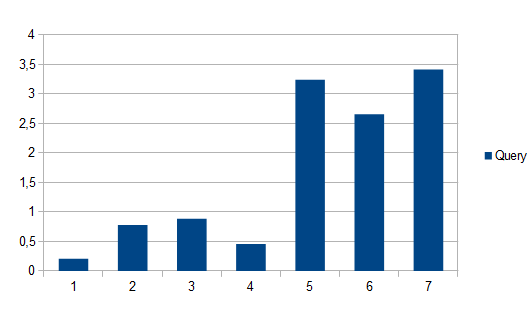
\includegraphics[width=1\textwidth]{fig1}
\\\textbf{Query 1}\\
SELECT * WHERE u.label() = 'switch', u.position = 'access'\\\\
2 simple selections, 0 joins. One pass through the vertices collection is enough to produce the result. 200 milliseconds evaluation time.
\\\\\\\textbf{Query2}\\
SELECT * WHERE (n) -[e with weight \textless 4]-\textgreater(m)\\\\
2 Joins and 1 Selection. The joins are not very expensive since we only use about 30\% of the edges. 700 milliseconds evaluation time.
\\\\\textbf{Query3}\\
SELECT * WHERE (n:switch) -\textgreater (m with position = 'distribution') \\\\
2 Joins and 2 Selections. I expected this query to be a little bit slower since we are using all the edges in the joins, but it is only a tiny bit slower than Query 2.
\\\\\textbf{Query4}\\
SELECT * WHERE (n with position = 'distribution') -[e with weight \textgreater 8]-\textgreater (m with position = 'access')\\\\
2 Joins and 3 Selections. Even though this query has more constraints than Query 2 and 3, it is faster since we only use 10\% of the edges in the joins. 
\\\\\textbf{Query5}\\
SELECT * WHERE (u WITH position = 'access') -\textgreater (v WITH position = 'distribution') -\textgreater (w WITH position = 'core')\\\\
4 Joins and 3 Selections. The last 3 queries all contain multiple query edges and are much slower. Since there is no selection on the edge, this particular query is quite slow even though it has "only" 4 joins..
\\\\\textbf{Query6}\\
SELECT * WHERE (u WITH position = 'access') -[e with weight  \textless 2]-\textgreater (v WITH position = 'distribution') -[f with weight \textgreater 8]-\textgreater (w WITH position = 'core')\\\\
4 Joins and 5 Selections. Like query 4, the evaluation time goes down as we add more constraints on the edges. Since we have a lot less tuples in the 3rd and 4th join, this query is faster than previous one.
\\\\\textbf{Query7}\\
SELECT * WHERE (u WITH position = 'access') -[e with weight  \textless 2]-\textgreater (v WITH position = 'distribution') -[f with weight  \textless 2]-\textgreater (w WITH position = 'core') -[g with weight  \textless 2]-\textgreater (x WITH position = 'distribution')\\\\
6 Joins and 7 Selections. This is probably the most interesting result. We add two more joins to the query, but we restrict the number of edges used in all the joins dramatically. This consequently leads to a surprisingly low evaluation time, almost on the level as query 5. This demonstrates how big the impact of the joins is for the evaluation time.
\\\\\textbf{Query 8}\\
SELECT * WHERE (u WITH position = 'access') -\textgreater (v WITH position = 'distribution') -\textgreater (w WITH position = 'core') -\textgreater (x WITH position = 'distribution')\\\\
6 Joins and 4 Selections. I have not included this query in the figure because the evaluation times are around 30 to 40 seconds when run with 48 workers. When using only a single worker I have measured evaluation times over 10 minutes. This is due to the fact that we join 6 times with the full edge collection.

\end{document}